%
% $RCSfile: polymorphism.tex,v $
%
% Copyright (C) 2002-2008. Christian Heller.
%
% Permission is granted to copy, distribute and/or modify this document
% under the terms of the GNU Free Documentation License, Version 1.1 or
% any later version published by the Free Software Foundation; with no
% Invariant Sections, with no Front-Cover Texts and with no Back-Cover
% Texts. A copy of the license is included in the section entitled
% "GNU Free Documentation License".
%
% http://www.cybop.net
% - Cybernetics Oriented Programming -
%
% http://www.resmedicinae.org
% - Information in Medicine -
%
% Version: $Revision: 1.1 $ $Date: 2008-08-19 20:41:08 $ $Author: christian $
% Authors: Christian Heller <christian.heller@tuxtax.de>
%

\subsubsection{Polymorphism}
\label{polymorphism_heading}
\index{Polymorphism}
\index{Method Overloading}
\index{Method Overriding}
\index{Super Class}
\index{Sub Class}
\index{super}

Another object oriented feature that comes with inheritance is
\emph{Polymorphism}. It allows methods to be \emph{overloaded} (sometimes
called \emph{overridden}). That is, on two objects created from different
classes inheriting from each other, the right equally named method will be
called by the language interpreter program (figure \ref{polymorphism_figure}),
which leads to different behaviour depending on the current object context.
Following is a \emph{Java} code example overloading a method to gain
polymorphic behaviour:

\begin{scriptsize}
    \begin{verbatim}
    public class super_class {
        public void method() {
            do_something();
        }
    }
    public class sub_class extends super_class {
        public void method() {
            do_something_else();
        }
    }
    \end{verbatim}
\end{scriptsize}

\begin{figure}[ht]
    \begin{center}
        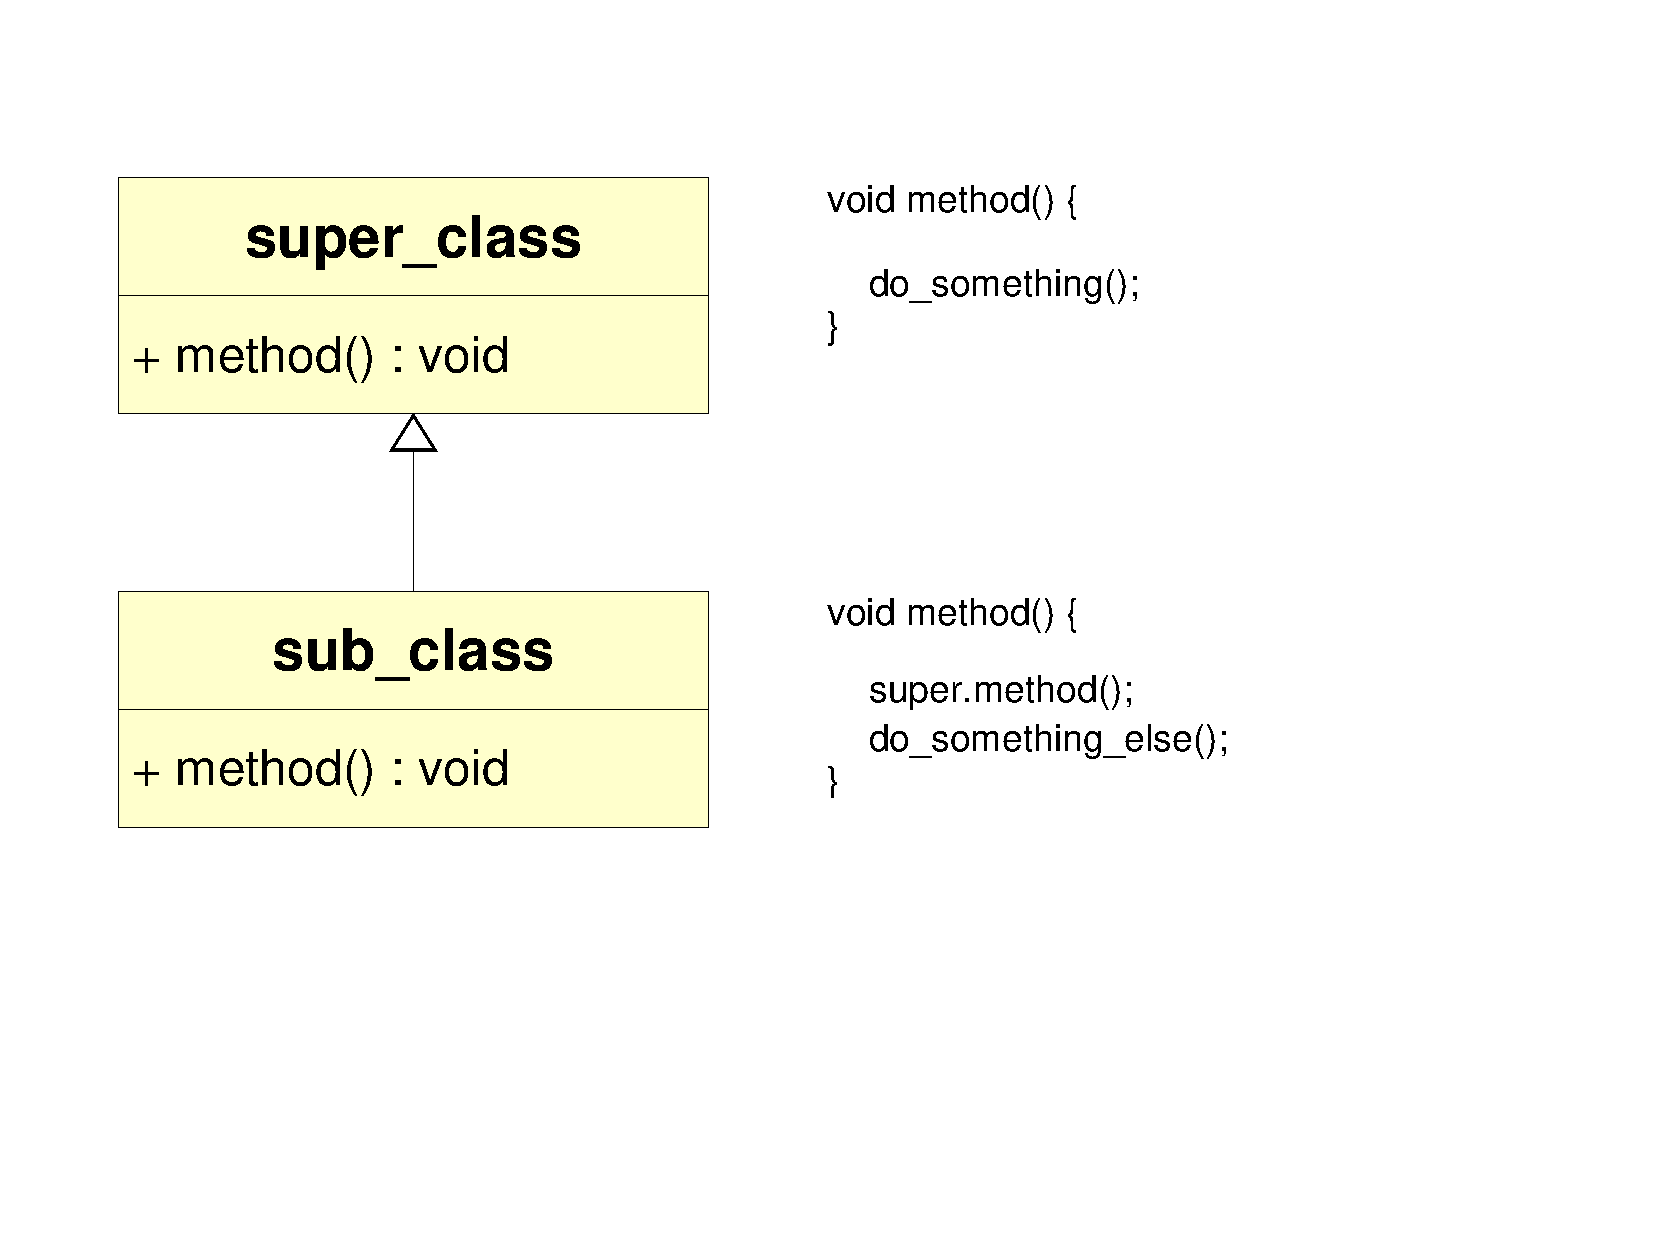
\includegraphics[scale=0.3,angle=-90]{graphic/polymorphism.pdf}
        \caption{Polymorphism as UML Diagram}
        \label{polymorphism_figure}
    \end{center}
\end{figure}

If objects instantiated from a sub class want to make use of the functionality
contained in the super class' equally named method, the sub class' method needs
to call the super class' method explicitly using the keyword \emph{super}:

\begin{scriptsize}
    \begin{verbatim}
    public class sub_class extends super_class {
        public void method() {
            super.method();
            do_something_else();
        }
    }
    \end{verbatim}
\end{scriptsize}
